\documentclass[12pt,a4paper]{article}
\usepackage{graphicx}
\usepackage[czech]{babel}
\usepackage[utf8]{inputenc}
\usepackage{titling}
\usepackage{pdfpages}
\usepackage[nopar]{lipsum}
\usepackage{mathtools}
\usepackage{multirow}
\usepackage{caption}
\usepackage{float}
\usepackage{enumitem}
\usepackage{listings}
\usepackage{amsmath}
\usepackage{amssymb}
\usepackage{url}
\usepackage[left=25mm,right=25mm,top=30mm,bottom=20mm]{geometry}
\bibliographystyle{abbrv}




\begin{document}
\title{SLAM - rešerše \\ Projekt 4}
\author{Jakub Kratochvíl}
\date{Akademický rok 2017/2018}
\begin{titlepage}
\begin{center}

\includegraphics[scale=0.5]{img/logo_zcu.png}\\
\vspace{5cm}
\begin{Large}
\textbf{\thetitle}\\
\end{Large}
\vspace{3cm}
\theauthor\\
\vspace{5cm}
\thedate
\end{center}
\end{titlepage}
\newpage
		
		
\tableofcontents
\newpage
\fontsize{12pt}{18pt}\selectfont


\section{Úvod}
SLAM je zkratka pro simultánní lokalizaci a mapování, jeden ze základních problémů autonomních robotů. Jeho řešením by měl být robot, schopný na neznámém místě v neznámém prostředí vytvořit mapu tohoto prostředí a zároveň se v ní sám během pohybu lokalizovat.

Do povědomí se SLAM dostal v roce 1986 na konferenci IEEE Robotics and Automation, která se konala v San Francisku v Kalifornii \cite{Durrant-Whyte}. V tomto období se v robotice a umělé inteligenci začaly objevovat metody založené na pravděpodobnostních principech a tak vyvstala otázka možnosti použití odhadových metod na mapovací a lokalizační problémy. Po následujících diskuzích se problém ukázal jako velice zajímavý a konzistentní pravděpodobnostní mapování se stalo jedním ze základních problémů a výzev robotiky.

Aplikací SLAM můžeme najít mnoho, počínaje autonomním domácím vysavačem nebo sekačkou na trávu přes robotický průzkum opuštěných nebo člověku nebezpečných prostor, navigaci ponorek kolem podmořských přírodních překážek, řízení bezpilotních letounů a dronů až po v poslední době hodně diskutované samořídící automobily nebo dokonce planetární rovery brázdící povrch Marsu.

Tato práce si klade za úkol čtenáře seznámit se základními vlastnostmi a popisem problému SLAM. Dává nahlédnout do jeho původní pravděpodobnostní definice a v další části se podrobněji zabývá metodou Graph SLAM. 


\newpage
\section{SLAM}
SLAM je problém týkající se otázky, zda je možné najít polohu nějakého zařízení vzhledem k jeho okolí a současně mapovat strukturu prostředí.

Landmarky nebo také majáky jsou nezaměnitelné a snadno rozpoznatelné orientační body v prostředí, které mohou být v některých aplikacích dopředu známy. Například autonomní vozík pohybující se ve výrobní hale může mít předem nadefinovanou mapu landmarků. Nebo robot pro práci pod širým nebem používající pro svou orientaci GNSS (globální družicový polohový systém). V takových případech, kdy lze stroj lokalizovat vzhledem ke známým bodům, nemusí být SLAM vyžadován. Ovšem v husté zástavbě, v podzemí a uvnitř budov je použití GNSS omezené nebo úplně nemožné. V neznámém prostředí zase nelze využít předem připravenou mapu a přichází nutnost použití jiného řešení, kterým bývá nejčastěji právě SLAM. Navíc v mnoha vojenských i civilních aplikacích není cílem lokalizace, ale právě robotem vytvořená mapa, kterou poté dále zpracovává lidský operátor.

Další z impulzů vývoje simultánní lokalizace a mapování byl špatný odhad pohybu získaný z odometrie kol, čímž se rozumí například počet otáček, úhel natočení apod. \cite{Past_Present_and_Future_of_Simultaneous_Localization_And_Mapping}. Tento odhad se navíc s ujetou vzdáleností zhoršuje (tzv. drift) a tím znemožňoval použití pro správnou a přesnou lokalizaci i tvorbu mapy. Nicméně dnešní algoritmy dokáží snížit drift na přijatelnou hodnotu 0,5\% a méně, takže v tomto ohledu není nutno využívat SLAM. \\ V čem je ale stále nenahraditelný, je schopnost tzv. uzavírání smyček. Při použití dat pouze z odometrie robot vnímá svět jako "nekonečný koridor", ve kterém neustále zkoumá nové oblasti (obr.1 vlevo). SLAM ale dokáže robotem vytvořenou smyčku uzavřít, protože porovná aktuální landmarky s těmi dříve objevenými a tím dokáže správně porozumět topologii prostředí a v mapě určit, že tyto dvě chodby se protínají (obr.1 vpravo). Levá mapa je vytvořená pomocí odometrie a znázorňuje jeden dlouhý koridor od bodu A do B. Body, které jsou ve skutečnosti blízko (B a C) mohou být podle této mapy libovolně daleko. Pravá mapa je vytvořená pomocí SLAM s využití uzavírání smyček, kde je znázorněná správná topologie prostředí, neboť robot správně našel "zkratku" mezi dvěma koridory \cite{Past_Present_and_Future_of_Simultaneous_Localization_And_Mapping}.

\begin{figure}[H]
\centering
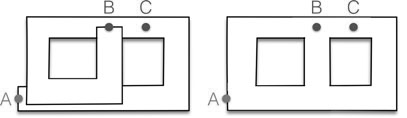
\includegraphics[scale=1]{img/Obr1_b} 
\caption{Levá část - odometrie, pravá část - SLAM} 
\end{figure}


\newpage
SLAM je ze své podstaty problém typu slepice-vejce a je tedy do značné míry netriviální. Robot pro svoji lokalizaci potřebuje mapu terénu, avšak k sestavení mapy musí znát svou vlastní polohu. Ovšem existují algoritmy, které, i přes tento rozpor, uspokojivě fungují a nasnadě je tedy otázka "Je SLAM vyřešen?". Ano i ne, otázku je nutno položit pro konkrétní konfiguraci robota, prostředí a požadavků, kde může figurovat mnoho kombinací, např. z následujících možností.
\begin{itemize}
\item Robot: dynamika, maximální rychlost, dostupné senzory, výpočetní výkon
\item Prostředí: 2D/3D, přírodní/umělé, přítomnost dynamických prvků, množství a typ landmarků, množství symetrie
\item Požadavky: přesnost odhadu stavu robota, přesnost a typ mapy, míra úspěšnosti, latence odhadu, maximální velikost mapované oblasti...
\end{itemize}
Například mapování vnitřního 2D prostředí s robotem vybaveným snímačem kol a laserovým senzorem s dostatečnou přesností a robustností lze považovat z velké části za vyřešené. Na druhou stranu další kombinace robot/prostředí/požadavky si stále zaslouží velké množství výzkumu. Aktuální algoritmy mohou snadno selhat, jestliže je pohyb robota nebo prostředí příliš náročný.


\subsection{Pravděpodobnostní definice}
Uvažujme mobilního robota, který se pohybuje v neznámém prostředí a pomocí svých senzorů pořizuje relativní pozorování okolních landmarků (obr.2).

\begin{figure}[H]
\centering
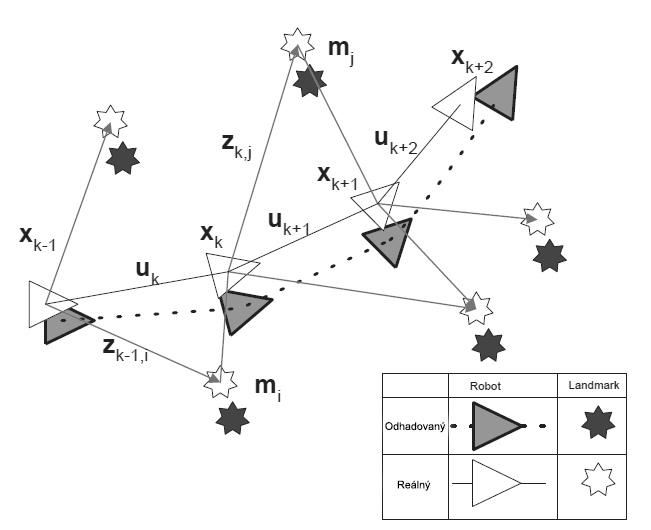
\includegraphics[scale=0.6]{img/Obr2_b}
\caption{Skutečné umístění landmarků ani robota není nikdy známo, jen jejich vzájemná poloha \cite{Durrant-Whyte}.}
\end{figure}

V okamžiku \textit{k} definujeme následující veličiny a zároveň vektory jejich historie od počátku snímání až do aktuálního časového kroku:
\begin{itemize}
\item \textbf{x}$_k$; \textbf{X}$_{0:k}=\lbrace \text{x}_0, \text{x}_1,\cdots, \text{x}_k\rbrace = \lbrace \textbf{X}_{0:k-1}, \textbf{x}_k \rbrace$:  
Stavový vektor popisující polohu a orientaci robota, respektive  historii všech jeho stavů.
\item \textbf{u}$_k$; \textbf{U}$_{0:k}=\lbrace \text{u}_1, \text{u}_2,\cdots, \text{u}_k\rbrace = \lbrace \textbf{U}_{0:k-1}, \textbf{u}_k \rbrace$: 
Vektor řízení použitý v čase \textit{k}-1 pro dosažení stavu x$_k$ v čase \textit{k}, resp. historie řízení.
\item \textbf{m}$_i$; $\textbf{m}=\lbrace \text{m}_1, \text{m}_2,\cdots, \text{m}_n\rbrace$: 
Vektor popisující polohu i-tého landmarku, resp. vektor popisující polohy všech landmarků.
\item \textbf{z}$_{ik}$; \textbf{Z}$_{0:k}=\lbrace \text{z}_1, \text{z}_2,\cdots, \text{z}_k\rbrace = \lbrace \textbf{Z}_{0:k-1}, \textbf{z}_k \rbrace$: 
Pozorování o poloze i-tého landmarku získané z robota, resp. soubor všech pozorování.
\end{itemize}

Skutečný robot bude vždy zatížen nějakou nepřesností použitých měřících zařízení a tak se přímo nabízí využití pravděpodobnosti pro formulaci úlohy SLAM. Tento přístup je jedním z nejběžnějších a také nejstarších. K vyřešení problému SLAM je potřeba určit sdruženou aposteriorní hustotu pravděpodobnosti landmarků \textbf{m} a stavů robota x$_k$ pro všechny časy $k$.

\begin{eqnarray}
p(\textbf{x}_k, \textbf{m} \,|\, \textbf{Z}_{0:k}, \textbf{U}_{0:k}, \textbf{x}_0)
\end{eqnarray}

K výpočtu je nutno znát vektor pozorování, vektor řízení a počáteční polohu robota. Výpočet hustoty se provádí pro každý časový okamžik $k$. Vhodné je použít rekurzivní algoritmus, který získá hustotu pravděpodobnosti v časovém okamžiku $k$ pomocí hustoty v okamžiku $k-1$.

\begin{eqnarray}
p(\textbf{x}_{k-1}, \textbf{m} \,|\, \textbf{Z}_{0:k-1}, \textbf{U}_{0:k-1})
\end{eqnarray}

Tento výpočet vyžaduje definování modelu pozorování a pohybového modelu.

\begin{enumerate}
\item \textbf{Model pozorování} popisuje s jakou pravděpodobností získáme pozorování z$_k$, pokud známe polohu robota i landmarků.
\begin{eqnarray}
p(\textbf{z}_k \,|\, \textbf{x}_k, \textbf{m})
\end{eqnarray}
\item \textbf{Pohybový model} popisuje s jakou pravděpodobností se robot nachází ve stavu x$_k$, pokud známe předchozí stav x$_{k-1}$ a aplikované řízení u$_k$.
\begin{eqnarray}
p(\textbf{x}_k \,|\, \textbf{x}_{k-1}, \textbf{u}_k)
\end{eqnarray}
\end{enumerate}

Stavový přechod pohybového modelu je Markovský proces, neboť stav x$_k$ závisí pouze na předchozím stavu x$_{k-1}$ a aplikovaném řízení u$_k$ a je nezávislý na pozorováních i mapě. SLAM algoritmus je nyní implementován ve standardní dvoustupňové (predikce-korekce) rekurzivní formě.

\newpage



\begin{enumerate}
\item \textbf{Predikce} 
\begin{eqnarray}
p(\textbf{x}_k, \textbf{m} \,|\, \textbf{Z}_{0:k-1}, \textbf{U}_{0:k}, \textbf{x}_0) \: = 
\end{eqnarray}
$$
= \: \int p(\textbf{x}_k \,|\, \textbf{x}_{k-1}, \textbf{u}_k) \: \times \: p(\textbf{x}_{k-1}, \textbf{m} \,|\, \textbf{Z}_{0:k-1}, \textbf{U}_{0:k-1}, \textbf{x}_0) d\textbf{x}_{k-1}  
$$
\item \textbf{Korekce}
\begin{eqnarray}
p(\textbf{x}_k, \textbf{m} \,|\, \textbf{Z}_{0:k}, \textbf{U}_{0:k}, \textbf{x}_0) \: = \: \frac{p(\textbf{z}_k \,|\, \textbf{x}_k, \textbf{m}) p(\textbf{x}_k, \textbf{m} \,|\, \textbf{Z}_{0:k-1, \textbf{U}_{0:k}, \textbf{x}_0})}{p(\textbf{z}_k \,|\, \textbf{Z}_{0:k-1}, \textbf{U}_{0:k})}
\end{eqnarray}
\end{enumerate}

Rovnice (5) a (6) poskytují rekurzivní postup pro výpočet hustoty pravděpodobnosti $p(\textbf{x}_k, \textbf{m} \,|\, \textbf{Z}_{0:k}, \textbf{U}_{0:k}, \textbf{x}_k)$ stavu robota \textbf{x}$_k$ a mapy \textbf{m} v čase $k$ na základě všech pozorování \textbf{Z}$_{0:k}$ a všech řízení \textbf{U}$_{0:k}$.

Problém budování mapy lze formulovat jako výpočet podmíněné hustoty pravdě\-podobnosti $p(\textbf{m} \,|\, \textbf{X}_{0:k}, \textbf{Z}_{0:k}, \textbf{U}_{0:k})$. To předpokládá, že umístění robota \textbf{x}$_k$ je známo (nebo alespoň deterministické) po celou dobu, pod podmínkou znalosti počátečního umístění. Mapa \textbf{m} se potom vytvoří spojením pozorování z různých míst. Naopak problém lokalizace může být formulován jako výpočet pravděpodobnostní distribuce $p(\textbf{x}_k \,|\, \textbf{Z}_{0:k}, \textbf{U}_{0:k}, \textbf{m})$. To předpokládá, že je známo umístění landmarků a cílem je vzhledem k nim vypočítat odhad umístění robota. Avšak model pozorování $p(\textbf{z}_k \,|\, \textbf{x}_k, \textbf{m})$ závisí jak na stavu robota, tak na umístění landmarků. Z toho vyplývá, že pravděpodobnostní hustota nelze takto rozdělit
$$
p(\textbf{x}_k, \textbf{m} \,|\, \textbf{z}_k) \: \ne \: p(\textbf{x}_k \,|\, \textbf{z}_k)p(\textbf{m} \,|\, \textbf{z}_k).
$$
Takové rozdělení by vedlo k nekonzistentnosti odhadů a nepoužitelným výsledkům. 

\section{Graph-Based SLAM}
Pravděpodobnostní přístup se v dnešní době již téměř nepoužívá, avšak na jeho základech staví všechny vyspělejší algoritmy. Jedním z nich je pravděpodobnostní SLAM, jehož hlavní myšlenka je založená na použití pravděpodobnostních filtrů. Z tohoto přístupu se vyvinul Graph SLAM, který je v mnoha ohledech lepší a rychlejší a bude hlavní náplní této práce. 

Při tomto přístupu se k ukládání dat používá graf. Uzel grafu reprezentuje stav robota a měření provedená z tohoto stavu. Hrany mezi uzly představují jejich vzájemnou polohu. Cílem algoritmu je najít takové rozložení uzlů, které minimalizuje čtvercovou chybu rozdílu pozorování a "virtuálního pozorování" \cite{GraphSLAM}. Tím se získá nejlepší odhad mapy. Optimalizace neprobíhá po každém novém pozorování, čímž se Graph SLAM řadí mezi offline metody řešení.

Formulace SLAM pomocí grafu byla poprvé představena v roce 1997, avšak kvůli vysoké výpočetní náročnosti trvalo ještě několik let, než se začala používat v reálných aplikacích. V dnešní době patří Graph SLAM k nejmodernějším technikám, co se rychlosti a přesnosti týče.

\subsection{Definice}
Pro správný chod graph SLAMu musí fungovat souhra mezi jeho dvěma částmi front-end a back-end. Front-end se obecně stará o sestrojení samotného grafu a back-end o jeho optimalizaci a tedy i optimalizaci mapy. Následující schéma znázorňuje průchod dat metodou Graph SLAM. Nezpracovaná data (pozorování, odometrie) nejdříve zpracuje front-end a vytvoří graf. Ten po daném okamžiku putuje do back-end, kde se optimalizací získá nejlepší odhad mapy prostředí a poté předá opět do první části \cite{16-graph-slam}.

\begin{figure}[H]
\centering
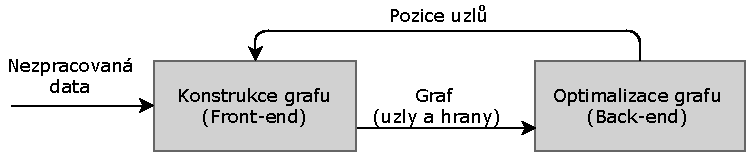
\includegraphics[scale=1.2]{img/Obr3.pdf}
\caption{Schéma toku dat v Graph SLAM}
\end{figure}

\subsubsection{Front-end}
První část vytváří graf, kterým reprezentuje mapu prostředí. Každý uzel $x_i$ obsahuje informaci o stavu robota a o pozorování provedeném z tohoto stavu v čase $i$. Hrana mezi sousedními uzly $x_i$ a $x_{i+1}$ odpovídá zaznamenané odometrii při pohybu robota. Pokud je hrana mezi různými uzly $x_i$ a $x_j$, pak je to tzv. virtuální měření. To se zaznamená ve chvíli, kdy robot naměří podobná data (tzn. ocitne se ve stejné části prostředí) jako v některém z předešlých měření. 

Využívá se scan matching, který porovnává dvě pozorování z uzlů $x_i$ a $x_j$ z různých časových okamžiků a v případě zjištění podobnosti je vypočítána relativní poloha uzlů $x_i$ a $x_j$. To je ve skutečnosti transformace pozorování z $x_i$ taková, aby se maximálně překrývalo s pozorováním uzlu $x_j$. Tuto transformaci nazýváme virtuálním pozorováním.

Znázornění problému je v obrázku 4, kde $x_i$ je aktuální uzel, $x_j$ je uzel, ve kterém bylo provedeno podobné pozorování jako to aktuální, $\hat{z}_{ij}$ je predikce virtuálního měření reprezentující "jak uzel $i$ vidí uzel $j$", $z_{ij}$ je virtuální měření, $\Omega_{ij}$ je informační matice virtuálního měření a $e_{ij}(x_i, x_j)$ je funkce, která vyjadřuje rozdíl virtuálního a predikovaného měření.
\begin{figure}[H]
\centering
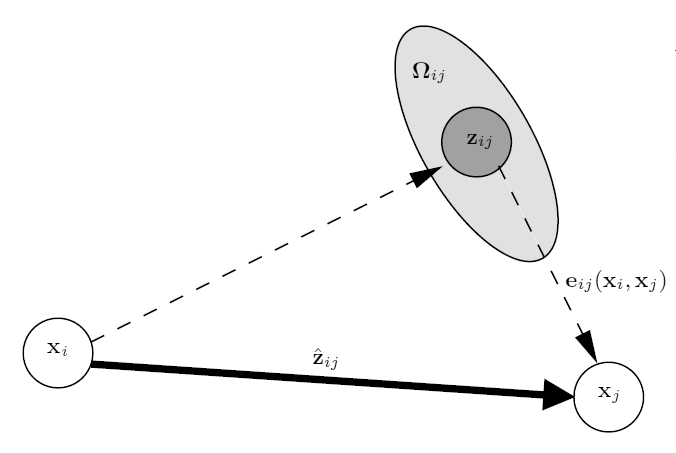
\includegraphics[scale=0.8]{img/Obr4_b}
\caption{Znázornění virtuálního měření a jeho predikce \cite{tutorialGraph}.}
\end{figure}



\subsubsection{Back-end}
Druhá část se stará o optimalizaci rozložení uzlů v grafu.

Definujme funkci 
$$
\textbf{e}_{ij}(\textbf{x}_i, \textbf{x}_j) \: = \: \textbf{z}_{ij}-\hat{\textbf{z}}_{ij}(\textbf{x}_i, \textbf{x}_j),
$$
která vyjadřuje chybu mezi predikcí měření $\hat{\textbf{z}}_{ij}$ a měřením $\textbf{z}_{ij}$ a je také znázorněna v obrázku 4. Optimalizace rozložení všech uzlů dosáhneme minimalizací funkce $\textbf{F}(\textbf{x})$ pro všechna virtuální měření
$$
\textbf{F}(\textbf{x}) \: = \: \sum\limits_{i,j} \textbf{F}_{ij} \: = \: \sum\limits_{i,j} \textbf{e}_{ij}^T \Omega_{ij} \textbf{e}_{ij}.
$$
Nejlepší odhad mapy tedy musí splňovat podmínku
$$
\textbf{x}^* \: = \: \text{argmin}\, \textbf{F}(\textbf{x}).
$$
Numericky lze tento problém řešit metodou nejmenších čtverců, konkrétně na odhad rozmístění uzlů z front-end aplikovat Gauss-Newtonův algoritmus, který minimalizuje chybovou funkci $\textbf{e}_{ij}(\textbf{x}_i, \textbf{x}_j)$.


\section{Vizuální SLAM}
Vizuální SLAM, Visual-based SLAM nebo také vSLAM je přístup k simultánní lokalizaci a mapování, při kterém jsou jako vstup algoritmu využívány obrazová data. Tato metoda se začala používat až po roce 2000, neboť zpracování obrazu z kamery je značně výpočetně náročné. 

Na druhou stranu sebou přináší dodatečné informace o vzhledu, barvě, jasu a textuře prostředí. To umožňuje začlenění dalších úkolů jako například detekce a rozpoznávání obličeje, věcí nebo konkrétních míst. Pro vSLAM také nahrává cenová dostupnost kamer, jejich velikost a nižší spotřeba energie oproti často používaným laserovým skenerům. 

Bohužel při použití snímačů obrazových dat mohou vzniknout chyby pokud kamera nemá dostatečné rozlišení, v prostředí je málo nebo moc landmarků, snímané povrchy nemají nedostatečnou texturu, málo osvětlení a jeho změny nebo pořízení rozmazaných snímků při pohybu. Navíc nezávisle na použitém algoritmu musí být provedena kalibrace kamer.

\subsection{Základní struktura vSLAM}
Většina vSLAM algoritmů používá stejnou obecnou strukturu, která se skládá ze tří hlavních částí:
\begin{itemize}
\item \textbf{Kalibrace} kamery 
\item \textbf{Sledování} a hledání společných bodů prostoru a mapy
\item \textbf{Mapování} - aktualizace a rozšiřování mapy
\end{itemize}

Nezávisle na přesném typu algoritmu musí proběhnout kalibrace kamer. Ta se dá rozdělit na vnitřní, která odpovídá geometrii kamery (ohnisková vzdálenost) a vnější, která záleží na pozici kamery v prostoru (rotace a translace s respektováním nějakého souřadnicového systému). Provádí se s použitím několika různých obrazů s motivem šachovnice. Jejich nasnímáním se vnitřní souřadnicový systém nastaví tak, aby odpovídal reálnému světu.

V další části je sledovaný obraz zasazen do rekonstruované mapy k odhadu pozice robota. K tomu je potřeba nejdříve najít společné významné body obrazu s mapou a poté vypočítat odhad pozice kamery.

Mapováním se rozumí rozšiřování existující mapy v případě, kdy kamera zachytí dosud neznámou oblast.

\subsection*{Dodatkové moduly vSLAM}
Následující dvě části jsou často zahrnuty do algoritmu pro stabilnější a přesnější běh, avšak v závislosti na konkrétním použití je lze vynechat:
\begin{itemize}
\item \textbf{Relokalizace} v případě ztráty povědomí o poloze
\item \textbf{Globální optimalizace mapy}
\end{itemize}

V případě, kdy robot ztratí přehled o své pozici, například kvůli rychlému pohybu kamery, je zapotřebí jej znovu lokalizovat. Pokud by vSLAM systém neobsahoval tuto funkci, nemohl by dále pokračovat po ztrátě informace o své pozici.

Mapa zpravidla obsahuje kumulativní chybu odhadu, která se zvětšuje s ujetou \linebreak vzdáleností. Když robot navštíví již dříve objevenou oblast, použitím techniky zvané uzavírání smyček, dojde k porovnání aktuálního obrazu s dříve nasnímanými obrazy a v případě shody může být dopočítána a následně odstraněna chyba odhadu.

\subsection{Metody řešení}
Existují tři základní přístupy v získávání a/nebo zpracování obrazových dat. První dva rozlišujeme podle práce s obrazovými daty, kdy jeden přístup je založen na detekci a zpracování významných bodů, zatímco druhý pracuje přímo se získaným obrazem. Třetí možností je použití RGB-D kamer jako je například Microsoft Kinect, který je výhodný v možnosti získávání nejen obrazu prostředí, ale i informaci o jeho hloubce. 

Tato práce se bude zabývat především monokulárním SLAMem, při kterém ke snímání prostředí používáme pouze jednu kameru. Výhody i nevýhody tohoto přístupu budou vysvětleny dále.

\subsubsection{S použitím významných bodů}
Metoda spočívá v zaznamenání vstupního obrazu a jeho převodu na významné body. Těmi jsou například různé hrany, snadno rozpoznatelné oblasti apod. Dále algoritmus pracuje pouze se získanými body a ne s celým obrazem. To zjednodušuje celkový problém, avšak je zde významné omezení v tom, že nedokážeme použít informaci z té části obrazu, která se nepřevede na nějaký významný bod a můžeme tím přijít o důležitá data, která by se dala lépe využít k odhadu mapy.

První monokulární SLAM nazvaný MonoSLAM byl vyvinutý v roce 2003. V tomto algoritmu probíhá lokalizace i mapování souběžně a k odhadu se používá Kalmanův filtr. Pohyb kamery a pozice významných bodů prostředí jsou reprezentovány stavovým vektorem. Při objevení nového významného bodu je tento přidán do stavového vektoru, v důsledku čehož se při použití ve velkém prostředí dimenze vektoru zvětší natolik, že výpočetní náročnost souběžné lokalizace a mapování přestává být únosná a je těžké dosáhnout potřebných odhadů v reálném čase. 

Řešením problému výpočetní náročnosti je lokalizaci a mapování spustit každé na svém vlastním procesorovém vlákně tak, jako v metodě zvané PTAM (tj. Parallel Tracking and Mapping). Tyto vlákna běží paralelně, tím nedochází k omezování lokalizace výpočetní náročností odhadu mapy. Navíc je do mapování zahrnuta i průběžná optimalizace, takže je robot v reálném čase lokalizován a navíc vytvářena přesná mapa prostředí. PTAM je první metodou, která zahrnuje optimalizaci do algoritmu v reálném čase a většina novějších algoritmů následuje tento vícevláknový přístup \cite{Taketomi_visual}.

PTAM, na rozdíl od MonoSLAM, dokáže v reálném čase fungovat i v případě rozlehlého prostředí, kde stavový vektor obsahuje několik tisíc významných bodů.

\subsubsection{RGB-D}
RGB-D SLAM se začal nejvíce používat po příchodu kamery Microsoft Kinect, která započala malou \uv{revoluci} díky své ceně, velikosti a jednoduchosti použití. Má zabudovanou RGB i infrakameru a dokáže tak kromě obrazu navíc získávat informaci o hloubce prostředí. Většina spotřebitelských RGB-D kamer je však určena pouze pro použití v interiéru, neboť v exteriéru je obtížné zachytit odražené IR záření a kromě toho mají malý dosah v řádu jednotek metrů.

Pomocí RGB-D kamer lze získat přímo 3D strukturu prostředí, většina přístupů však mapu rekonstruuje z kombinací více hloubkových map. K odhadu pozice kamery je hojně využívaný iterativní algoritmus nejbližšího bodu (ICP). 

\subsubsection{Přímé metody}
Přímé metody zpracovávají vstupní obraz bez použití doplňků extrahujících určité části obrazu a používají tak jeho fotometrickou konzistenci (metody s detekcí významných bodů využívají geometrické konzistence obrazu). Tímto přístupem získáme podstatně více informací o geometrii prostředí, které mohou být užitečné pro lokalizaci a mapování.

Jedním příkladem je metoda DTAM, kde při lokalizaci porovnáváme vstupní obraz s uměle generovaným obrazem z rekonstruované 3D mapy. Tento algoritmus bývá implementován na grafické kartě, čímž dosáhneme vyšší efektivity výpočtu a zároveň oddělení lokalizace a mapování. Mapování se provádí s využitím několika sérií pozorování z různých míst a následnou optimalizací. Tímto způsobem lze získat všechny 3 souřadnice každého pixelu a sestavit tak 3D mapu prostředí. DTAM je navržený pro rychlé a online 3D modelování pro použití s mobilním telefonem.

Další přímé metody budou podrobně vysvětleny ve zvláštní kapitole.

\subsection{Monokulární vSLAM}
Jedním z hlavních důvodů používání SLAMu s jedinou kamerou je malá náročnost na používaný hardware. Je mnohem levnější a menší než například stereo SLAM. Oproti použití dvou kamer nevyžaduje kalibraci jejich vzájemné polohy. Velká výhoda je také v možnosti použití s mobilními smartphony, které mají obvykle jednu kameru a tím pádem vše, co je potřeba k běhu algoritmu. Není zapotřebí žádného externího hardwaru a SLAM se tím stává snadno dostupným.

Na druhou stranu nevýhodou je nemožnost získání informace o hloubce prostředí z jednoho pozorování. Tuto informaci je potřeba dopočítat analýzou několika pozorování z různých míst. Algoritmy jsou více komplikované a také výpočetně náročné.

\section{Konkrétní přímé metody}
Dále se bude práce zabývat pouze přímými metodami řešení úlohy vizuální lokalizace a mapování. Nejdůležitější z nich budou podrobněji popsány v této kapitole.

\subsection{Semi-Dense Visual Odometry}
Tato metoda je pouze vizuální odometrií a není tedy určená pro sestavování globální mapy prostředí, ale přišla s přístupem, na kterém staví některé následující metody, které již jsou plnohodnotnými SLAM algoritmy. Klíčovou myšlenkou je průběžně odhadovat polo-hustou inverzní hloubkovou mapu pro aktuální snímek, která se dále používá pro sledování pohybu kamery pomocí zarovnání obrazu. Polo-hustou se rozumí hloubková mapa, která neobsahuje hloubkovou informaci pro každý pixel, ale pouze pro podmnožinu pohybujících se pixelů (mají nezanedbatelný obrazový gradient). Tím se značně sníží výpočetní náročnost oproti použití husté hloubkové mapy. Každý odhad je reprezentován jako Gaussovo rozdělení pravděpodobnosti nad inverzní hloubkou. Tyto informace jsou navíc aktualizovány v průběhu času při příchodu nových snímků. Celý algoritmus běží v reálném čase na CPU.

\subsubsection*{Odhad hloubkové mapy}
Hlavní částí tohoto algoritmu je odhad polo-husté inverzní hloubkové mapy pro aktuální obraz, která může být použita pro odhad pozice kamery u následujícího snímku. Tato mapa se průběžně šíří ze snímku do snímku a zpřesňuje se novými hloubkovými měřeními. Ty získáváme porovnáním jednotlivých pixelů s použitím adaptivní základní čáry (tzv. baseline) u minimálně dvou prostorově posunutých snímků. To umožňuje přesně odhadnout hloubku blízkých i vzdálených částí obrazu. Je vhodné použití více délek baseline, neboť pomocí krátké baseline určíme jednu hodnotu hloubky, avšak ne příliš přesně. Při použití dlouhé baseline dostáváme více přesných hodnot. Jejich kombinací lze dosáhnout správné a přesné hodnoty hloubky pixelu.

\begin{figure}[H]
\centering
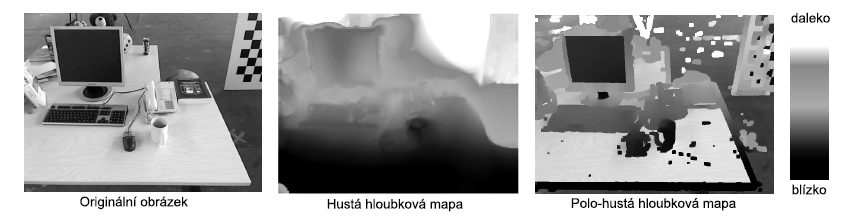
\includegraphics[scale=0.7]{img/hloubkova_mapa.jpg}
\caption{Ukázka polo-husté hloubkové mapy \cite{Semi-Dense_VO}.}
\end{figure}

\begin{figure}[H]
\centering
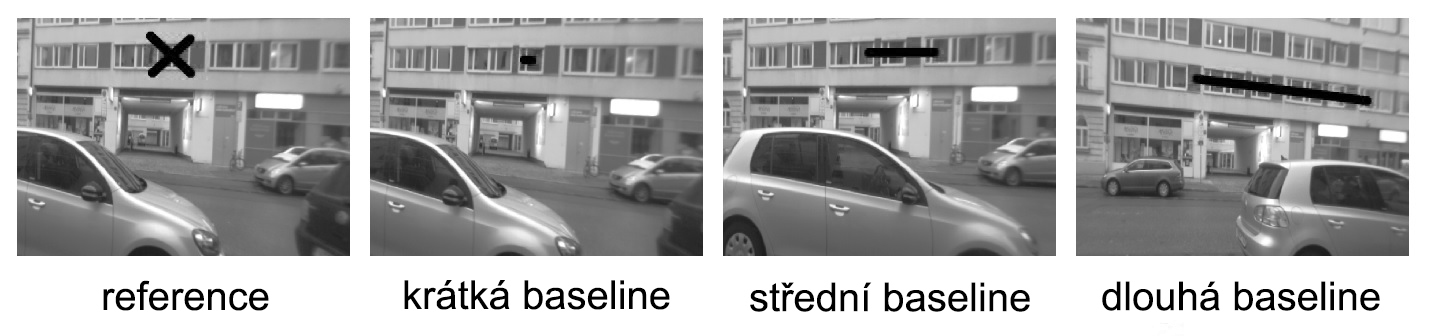
\includegraphics[scale=0.4]{img/baseline.jpg}
\caption{Ukázka pojmu baseline na reálných datech \cite{Semi-Dense_VO}.}
\end{figure}

\subsubsection*{Aktualizace hloubkové mapy}
Celková aktualizace hloubkové mapy se provádí jednou pro každý nový snímek a skládá se z následujících kroků: Nejprve je vybrána podmnožina obrazových bodů, pro kterou je přesnost vyhledání rozdílu dostatečně velká. Pro každý pixel se pak jednotlivě vybere vhodný referenční snímek a provede se jednorozměrné hledání rozdílnosti. Dřívější poznatky, pokud je to možné, se používají ke snížení rozsahu rozdílového vyhledávání a tím zmenšení výpočetních nákladů a odstranění falešných minim. Získaný inverzní hloubkový odhad se poté spojí do hloubkové mapy.

S výběrem referenčního snímku pomáhá zavedení jednoduché heuristiky. Použijeme nejstarší snímek, v němž byl pozorován pixel a jeho rozdílnost a pozorovací úhel nepře\-sahují určitou stanovenou mez. Pokud není nalezena dobrá shoda, \uv{věk} pixelů se zvýší, takže následné vyhledávání používá novější snímky, kde je větší pravděpodobnost, že pixel bude stále viditelný.


\subsubsection*{Shrnutí}
Sledování a odhad hloubky běží na dvou samostatných vláknech. Jedno průběžně propaguje inverzní hloubkovou mapu k nejnovějšímu zpracovávanému snímku, aktualizuje ji a částečně upravuje. Druhé současně sleduje každý příchozí snímek na nejnovější dostupné hloubkové mapě. Zatímco sledování je prováděno v reálném čase na 30Hz, jedna úplná iterace mapování trvá déle a je prováděna zhruba na 15Hz. Pokud je mapa složitá, adaptivně snižujeme počet stereo porovnání, abychom udrželi konstantní kmitočet. U stereo pozorování je zachována vyrovnávací paměť až 100 posledních snímků, která automaticky odstraňuje ty, které jsou používány nejméně.

Je použita standardní metoda založená na klíčových bodech pro získání relativní pozice kamery mezi dvěma počátečními snímky, které se pak používají k inicializaci inverzní hloubkové mapy. Po proběhnutí této inicializace je metoda zcela samostatná. Ve většině případů je algoritmus dokonce schopen zotavit se z náhodných nebo extrémně nepřesných počátečních hloubkových map, což naznačuje, že inicializace založená na klíčových bodech by se mohla v budoucnu stát nadbytečnou.

\subsection{LSD-SLAM}
Metoda LSD-SLAM (Large-Scale Direct monocular SLAM) umožňuje vytvářet konzistentní rozsáhlé mapy prostředí. Používá přímé zpracování vstupního obrazu spolu s odhadem založeným na filtraci polo-hustých hloubkových map, které přinesla zmiňovaná metoda Semi-Dense Visual Odometry \cite{Semi-Dense_VO}. Globální mapa je reprezentována jako graf, jehož vrcholy představují vstupní obrazy a 3D transformace podobnosti znázorňují hrany umožňující detekci a opravu nahromaděné chyby. Metoda běží v reálném čase na CPU a jako odometrie i na smartphonu.

\subsubsection*{Přehled metody}
Algoritmus se skládá ze tří hlavních částí:
\begin{itemize}
	\item \textbf{Sledování} průběžně monitoruje nové obrazy z kamery a odhaduje jejich pozici vzhledem k aktuálnímu snímku. Přitom používá pozici předchozího snímku jako vlastní inicializaci. 
	\item \textbf{Odhad hloubkové mapy} využívá sledované snímky k úpravě nebo nahrazení aktuálního snímku. Hloubka je získána filtrací mnoha prostorových porovnání pixelů s použitím krátké baseline, stejně jako v metodě Semi-Dense Visual Odometry. Při velkém posunu kamery se nový snímek inicializuje promítnutím bodů z aktuálního snímku do snímků z jeho blízkého okolí. 
	\item \textbf{Optimalizace mapy} se provádí nejdříve ve chvíli, kdy je u aktuálního snímku ukončen jeho hloubkový odhad. Pro detekci uzavření smyčky anebo chyby měřítka je s použitím zarovnání obrazu odhadována podobnostní transformace snímku se snímky v jeho blízkém okolí.
\end{itemize}

\paragraph{Inicializaci} prvního snímku je doporučeno provést náhodnou hloubkovou mapou s velkou variancí. Při dostatečném translačním pohybu kamery v prvních sekundách algoritmus sám konverguje ke správné hloubkové konfiguraci.

\paragraph{Mapa} je reprezentována jako graf. Každý vrchol grafu obsahuje snímek z kamery, inverzní hloubkovou mapu a její varianci, které jsou definovány pouze pro podmnožinu pixelů (a jejich blízkého okolí) s největším obrazovým gradientem. Hrany mezi vrcholy obsahují informaci o vzájemné relativní poloze vrcholů a odpovídající kovarianční matici.

\paragraph{Unikátnost} LSD algoritmu stojí na tom, že to byl první přímý monokulární SLAM, zatímco jeho \uv{předchůdci} dělaly pouze vizuální odometrii \cite{Engel14_LSD}. K tomu zřejmě pomohla i nová metoda zarovnání snímků s různým měřítkem. 

Při použití jediné kamery nelze z principu pozorovat absolutní měřítko sledovaného prostoru, to vede, zejména u delších trajektorií, k hromadění chyby měřítka a chybnému fungování celého algoritmu. LSD SLAM tento problém řeší s použitím vnitřní korelace mezi hloubkou scény a přesností sledování. Hloubková mapa každého klíčového snímku je normována tak, že střední inverzní hloubka je rovna jedné. Tak je možné do transformací mezi snímky začlenit i rozdíl jejich měřítek, ve výsledku explicitně vyjádřit velikost nahromaděné chyby a adekvátně upravit absolutní měřítko celé mapy.

\subsection{Direct Sparse Odometry}
DSO je přímou vizuální odometrií, postavená na využití vysoce přesné řídké hloubkové mapy. Díky tomu je první plně přímou metodou, která dokáže v reálném čase optimalizovat pravděpodobnosti všech získávaných parametrů (pozice kamery, vnitřní parametry kamery a geometrii prostředí, respektive jeho inverzní hloubku). Oproti tomu například zmiňovaná metoda Semi-Dense Visual Odometry používá nepřímou formulaci k optimalizaci parametrů.

Z hlediska přesnosti sledování i robustnosti výrazně překonává i nejmodernější použí\-vané přímé a nepřímé metody v různých reálných podmínkách. Při použití v reálném čase hravě předčí hlavní nepřímé metody a při vysokém nastavení (více bodů a aktivních klíčových snímků) vytváří podobně husté, avšak daleko přesnější modely prostředí než LSD SLAM \cite{Engel2018_DSO}.

\subsubsection*{Řídká hloubková mapa} Mapa je sestavena pouze z vybrané sady nezávislých bodů (tradičně rohů). Oproti metodám využívající husté hloubkové mapy, které se k její tvorbě snaží použít všechny nasnímané pixely. Třetí možností kombinující oba přístupy jsou již dříve zmiňované polo-husté hloubkové mapy, které nepoužívají celý obraz, avšak stále se zaměřují na využití propojených a dobře ohraničených podmnožin. 

Kromě rozsahu použité oblasti obrazu je zde významnější rozdíl v přidání apriorní informace o geometrii prostředí. Neexistuje zde žádná definice sousedních pixelů a pozice klíčových bodů jsou tak nezávislé k poloze kamery. Nevýhodou přidání této informace je možnost zanesení zkreslení a tím snížení přesnosti 3D rekonstrukce rozsáhlých prostředí. 

\subsubsection*{Optimalizace} Provádí se s pomocí klouzavého okna, kdy staré pozice kamery a body, které opustí toto okno jsou v úloze již ignorovány. Na rozdíl od ostatních přímých metod simultánně optimalizuje všechny parametry modelu, při udržení stejné geometrické reprezentace používanou jinými přímými přístupy.

Navržený model umožňuje některá pozorování použít vícekrát, zatímco jiné nepoužít vůbec. Stává se to z důvodu umožnění překrytí bodových pozorování (a tedy více pozorování závisí na stejných hodnotách pixelů), přestože strategie výběru bodů se tomu snaží zabránit rovnoměrným rozložením bodů v prostoru. Děje se tak zejména ve scénách s nízkou texturou, kde musí být všechny body vybrány z relativně malé oblasti s texturovaným obrazem. 

\subsubsection*{Správa snímků}
Metoda stále drží klouzavé okno maximálně \textit{N} aktivních snímků (standardně \textit{N} = 7). Každý nový snímek je zpočátku sledován s respektem k těmto referenčním snímkům.

\paragraph*{1) Počátek sledování nových snímků.} Při inicializaci nového klíčového snímku jsou do něj promítnuty a mírně rozšířeny všechny aktivní body a tím vytvořena polo-hustá hloubková mapa. Nové snímky jsou sledovány s ohledem pouze na tento klíčový snímek. Obrázek 7 ukazuje některé příklady inicializace hloubkové mapy. Zároveň je zde dobře vidět používaná hustota hloubkové mapy, kde další zvyšování hustoty by vedlo pouze k minimálnímu zlepšení přesnosti a robustnosti, avšak by významně zpomalilo běh algoritmu. Za povšimnutí stojí rozložení stejného počtu hloubkových bodů. V hustě texturovaných prostředích (vlevo) jsou rozprostřené po celém snímku, zatímco při malé části texturovaného obrazu jsou rozloženy podobně jako v LSD SLAMu.

Předpokládá se, že selhalo přímé zarovnání obrazu, pokud je střední kvadratická odchylka aktuálního snímku větší nebo rovna dvojnásobku odchylky předchozího snímku. Poté se metoda snaží obnovit novou inicializací provedením až 27 různými malými rotacemi v různých směrech. Každý takový pokus trvá přibližně 0,5ms, ale je potřeba jen velmi zřídka, a to v případech, kdy se kamera pohybuje velmi rychle nebo roztřeseně.

\begin{figure}[H]
\centering
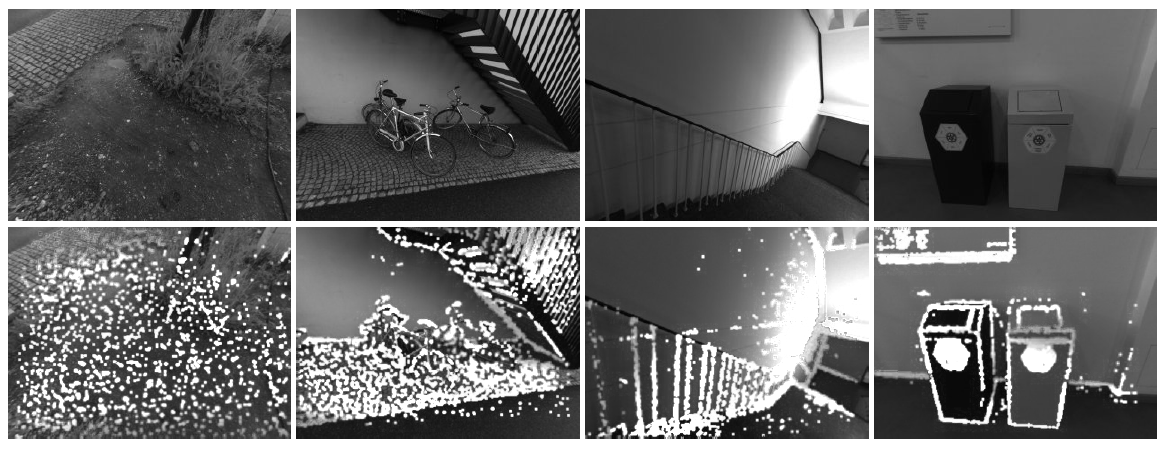
\includegraphics[scale=0.64]{img/Obr5_b.png}
\caption{Příklady hloubkových map. V horní řadě jsou originální snímky, v dolní snímky s promítnutými hloubkovými mapami.  \cite{Engel2018_DSO}.}
\end{figure}

\paragraph*{2) Vytváření klíčových snímků.} Metoda zpočátku vytvoří několik klíčových snímků (přibližně 5-10 za vteřinu) a poté je vytřídí marginalizací nadbytečných snímků. Kombinují se zde 3 pravidla k rozhodnutí, zda je třeba vytvořit nový klíčový snímek:
\begin{itemize}
\item První pravidlo sleduje změnu zorného pole, kterou reprezentuje střední kvadratický optický tok z posledního klíčového snímku do posledního snímku
 
\( f:=(\frac{1}{n}\sum_{i=1}^n||\textbf{p}-\textbf{p}'||^2)^\frac{1}{2} \), kde \textbf{p} je fotometrická chyba a \(\textbf{p}'\) je promítnutá pozice \textbf{p} s inverzní hloubkou.

\item Vyšší počet vytvořených klíčových snímků vyžaduje posun kamery, který je měřen středním optickým tokem bez rotace \( f:=(\frac{1}{n}\sum_{i=1}^n||\textbf{p}-\textbf{p}'_t||^2)^\frac{1}{2} \), kde \(\textbf{p}'_t\) je \(\textbf{p}'\) bez rotace.

\item Nový klíčový snímek je vytvořen pokud se významně změní expoziční čas kamery, ten je měřen jako relativní jas mezi dvěma snímky \( a:=|\log(e^{a_j-a_i} t_j t_i^{-1})| \), kde \( e \) je afinní jasová transformační funkce \cite{Engel2018_DSO}.
\end{itemize}


\paragraph*{3) Marginalizace starých klíčových snímků.} Nechť \( I_1 \dots I_n \) je množina aktivních klíčových snímků seřazených od nejnovějšího po nejstarší.
\begin{itemize}
\item Dva nejnovější klíčové snímky \( I_1 \) a \( I_2 \) vždy ponecháváme.
\item Všechny snímky s méně než 5\% podílem bodů viditelných v \( I_1 \) jsou marginalizovány.
\item Pokud je počet aktivních klíčových snímků větší než \( N_f \), marginalizujeme snímek s nejvyšší funkční hodnotou \( s(I_i) \). \( s(I_i)=\sqrt{d(i,1)} \sum_{j=3}^n (d(i,j)+\epsilon)^{-1}, j\neq i \), kde \( d(i,j) \) je eukleidovská vzdálenost mezi snímky \( I_i \) a \( I_j \) a \( \epsilon \) je  malá konstanta. Tato funkce je heuristicky vytvořená pro zachování správného rozdělení snímků v prostoru, s vyšším důrazem na snímky blízké aktuálnímu snímku.
\end{itemize}

\subsubsection*{Správa bodů}
Většina přímých metod se snaží využívat co nejvíce dostupných obrazových dat, avšak k udržení běhu algoritmu v reálném čase jsou nuceny akumulovat nedokonalé odhady a aproximovat, nebo ignorovat, korelace mezi jednotlivými parametry. Namísto toho DSO využívá silně podvzorkovaná data, díky čemuž je lze v reálném čase řádně optimalizovat. Experimenty navíc dokazují, že obrazová data jsou silně redundantní a využití většího množství dat není zásadní výhodou. 

Metoda se vždy snaží držet pevný počet \( N_p \) aktivních bodů (standardně \( N_p = 2000 \)) rovnoměrně rozložených napříč prostorem a aktivními snímky. V každém klíčovém snímku je vybráno \( N_p \) kandidátních bodů, které jsou následně sledovány a případně přidány do optimalizace. V případě potřeby přidat do optimalizace nové body vybíráme z kandidátních bodů, kterých je díky tomuto přístupu (\( N_p \) kandidátních bodů v každém snímku, ale pouze \( N_p \) aktivních bodů ve všech aktivních snímcích) vždy dostatek i přesto, že některé z nich již můžou být neplatné.

\paragraph*{1) Výběr kandidátních bodů.} Zaměřujeme se na body, které jsou dobře rozložené v obraze a mají dostatečně vysoký gradient vzhledem k jejich bezprostřednímu okolí. Regionální prahovou hranici pro rozhodnutí o dostatečně vysokém gradientu získáme rozdělením obrazu na \( 32 \times 32 \) bloků a pro každý zvlášť vypočítáme hodnotu jeho prahu.

Abychom dosáhli stejného rozdělení bodů, rozdělíme obraz na \( d \times d \) bloků a z každého vybereme bod s nejvyšší hodnotou gradientu (pokud převyšuje regionální práh). Někdy je ovšem prospěšné zahrnout i body z oblastí se slabším gradientem, které mohou zachycovat například informaci o hladce se měnící intenzitě osvětlení na bílé stěně. Proto tento postup opakujeme ještě dvakrát se sníženým gradientním prahem a blokovou velikostí \( 2d \) a \( 4d \). Velikost bloku \( d \) se může v průběhu algoritmu měnit podle počtu již vybraných bodů, tzn. jeho zvětšení, pokud je již vybráno hodně bodů a naopak.

\paragraph*{2) Sledování kandidátních bodů.} V následujících snímcích jsou kandidátní body sledovány s použitím diskrétního vyhledávání podél epipolární přímky \cite{Engel2018_DSO}. Z nejlepší shody je vypočítána hloubka a související variance, která je používána k omezení vyhledávání u následujících snímků. Body, které nejsou navzájem dostatečně odlišné jsou vyřazeny, to výrazně snižuje počet falešných shod v opakujících se oblastech. Vypočítaná hloubka slouží pouze jako inicializace pro aktivaci bodu.

\paragraph*{3) Aktivace kandidátních bodů.} Po marginalizaci souboru starých bodů jsou aktivovány kandidátní body. Do nejnovějšího klíčového snímku jsou promítnuty aktivní i kandidátní body a z nich jsou aktivovány ty, které maximalizují vzdálenost k nějakému existujícímu bodu.

\subsection{Direct Sparse Odometry with Loop Closure}
Zkráceně LDSO je rozšířením popsaného Direct Sparse Odometry (DSO) o uzavírání smyček a optimalizaci pozic robota. Tím se z LDSO stává plnohodnotná SLAM metoda.

Typický vizuální SLAM se skládá z frontend, starajícího se o sledování pohybu kamery a backend, který vytváří a spravuje mapu prostředí a zmenšuje nahromaděnou chybu pomocí uzavírání smyček a globální optimalizace. LDSO přišlo s nápadem přizpůsobit DSO k použití na frontend pro odhad vizuální odometrie a v backend části dělat korekci její chyby s využitím uzavírání smyček a optimalizace mapy. Přičemž samotný DSO se již skládá ze svého frontend a backend. Tento přístup je vhodný například pro vyčíslení fotometrické chyby, neboť za normálních okolností by musely být v paměti uchovány obrazy minulých klíčových snímků a při začlenění měření z těchto snímků do výpočtu je obtížné zajistit konzistenci odhadu, protože stejná obrazová informace je již použita v marginalizaci a neměla by být používána znovu. Navíc zakomponování uzavírání smyček díky minimalizaci chyb translace, rotace a měřítka otevírá možnosti použití algoritmu v rozsáhlejších prostředích.

Detekce smyček je v nepřímých vizuálních metodách nejčastěji založena na indexování významných částí obrazu (například metoda Bag of words, která části obrazu reprezentuje slovy a celý obraz histogramem těchto slov) a je snadno aplikovatelná na nepřímou vizuální odometrii opětovným použitím významných částí obrazu z fronted. V přímých metodách to však není tak jednoduché. Pokud budeme detekovat a porovnávat části obrazu nezávisle odděleně od fronted, nemusíme získat hloubkové odhady bodů potřebných pro efektivní výpočet pozičních omezení robota. Naopak při pokusu znovu použít body z fronted a vypočítat pro ně identifikátory, pravděpodobně nebudou odpovídat opakujícím se částem obrazu a vedou ke špatné detekci uzavření smyčky. Vizuální odometrie byly v minulosti rozšiřovány na SLAM buď za použití porovnání podobnosti klíčových snímků a následné vyhodnocení uzavření smyček, nebo výpočty důležitých částí obrazu odděleně od fronted. To vyžaduje dostupnost klíčových snímků po celou dobu běhu algoritmu. LDSO namísto toho navrhuje, aby výběr bodů směřoval k opakovatelně použitelným částem obrazu a použití geometrických funkcí k výpočtu pozičních omezení.

\paragraph*{Souhrn provedených vylepšení:}
\begin{itemize}
\item Strategii bodového výběru DSO přizpůsobujeme tak, aby byla zajištěna možnost opakovaného použití rohových klíčových bodů a zároveň zachována robustnost v slabě texturovaných prostředích. Vybrané rohové prvky jsou poté použity pro detekci uzavření smyčky s použitím Bag of words.
\item Využíváme hloubkových odhadů odpovídajících si klíčových bodů pro výpočet \newline pozičních omezení v kombinaci s poziční optimalizací, zarovnání mračna bodů a překrytím grafem relativních pozic získaných z optimalizovaného posuvného okna z DSO.
\item Na veřejně dostupných souborech dat demonstrujeme, že bodový výběr zachovává přesnost i robustnost a optimalizace grafu pozic významně snižuje chybu odometrie a vede k výkonu srovnatelnýmu s nejlepšími nepřímými metodami i bez použití globální optimalizace.
\end{itemize}

Na obrázku 8 lze vidět rozdíl po detekci a uzavření smyčky ve veřejně dostupných datech z Technické univerzity Mnichov. Černou barvou je trajektorie před uzavřením a bílou po uzavření smyčky. V přiblížených výřezech lze vidět vylepšení zarovnání mračna bodů.

\begin{figure}[H]
\centering
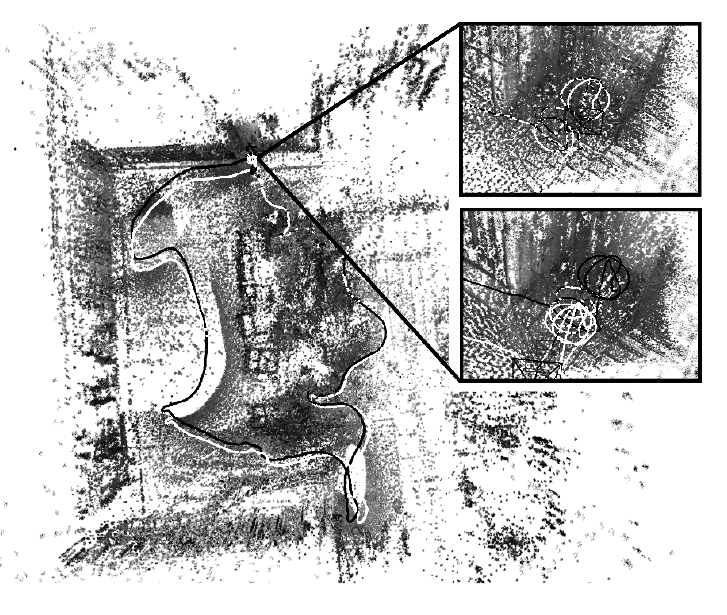
\includegraphics[scale=0.75]{img/Obr6_b.png}
\caption{Ilustrace jak LDSO zmenší nahromaděnou chybu po uzavření smyčky.\cite{LDSO}.}
\end{figure}

\subsubsection*{Uzavírání smyček}
Pro dlouhodobé uzavírání smyček v DSO je zapotřebí zavést globální optimalizační linku zajišťující vyhledávání a validaci smyček. Kvůli nutnosti ukládání všech obrazů a velkému množství bodů v 3D mapě bylo zavrženo použití globální fotometrické optimalizace a místo toho zvolena optimalizace grafu pozic. Vedle okna DSO přidáme globální poziční graf, abychom udrželi spojení mezi klíčovými snímky. Z posuvného okna DSO přebereme relativní 3D transformace pozic mezi klíčovými snímky. Pro detekci a validaci smyček spoléháme na metodu Bag of words. Pokud je kandidát smyčky schválen, je vypočtena jeho vazba s ohledem na aktuální klíčový snímek a přidána do globálního grafu pozic, který je poté optimalizován pro zpřesnění dlouhodobého odhadu pozice robota.

Přímé metody, na rozdíl od nepřímých, při výběru bodů nevyžadují jejich opakovatelné použití, které je ale vhodné pro hledání shody obrazu v problému uzavírání smyček. DSO používá dynamické vyhledávání v mřížce pro získání dostatečného počtu pixelů i ve slabě texturovaných prostředích. Tuto strategii v LDSO upravujeme tak, aby byla citlivější na rohové body při zachování potřebného počtu pixelů (standardně 2000). Vizuální odometrie v frontend používá jak rohové, tak nerohové pixely pro sledování pohybu kamery, čímž udržuje dodatečnou režii pro extrakci důležitých částí obrazu z vlákna pro uzavírání smyček na minimu.

\subsubsection*{Shrnutí}
LDSO ukazuje možný přístup začlenění uzavírání smyček a globální mapovou optimalizaci do přímé vizuální odometrie. Výběr bodů z DSO je přizpůsoben tak, aby zahrnoval znovu použitelné části obrazu. Pro ty jsou následně vypočítány identifikátory a vytvořeny modely metodou Bag of words pro detekci smyček. Tyto změny zachovávají robustnost a přesnost původní odometrie, přičemž snižují globální chybu rotace, posuvu i měřítka \cite{LDSO}.


\section{Porovnání metod}
V této kapitole je vysvětlen způsob zprovoznění čtyř vybraných metod provádějících přímou vizuální odometrii, nebo přímý vizuální SLAM - Semi-Direct Visual Odometry (SVO), LSD-SLAM, Direct Sparse Odometry (DSO) a Direct Sparse Odometry with Loop Closure (LDSO). Dále jsou zde popsána testovací data, jejich úpravy, použití a následné získání výsledných dat z jednotlivých metod. Je zde popis potřebných úprav trajektorií pro vyhodnocení jejich vlastností, vykreslení a celkové porovnání.

\subsection{Robot Operating System}
Mnoho metod pro lokalizaci a mapování je uzpůsobeno na provozování s pomocí ROS, což je balík knihoven a nástrojů vytvořený pro snadnější vývoj robotického softwaru. ROS není tradiční operační systém, jak by se mohlo z názvu zdát, je často označovaný jako \uv{middleware} a nelze ho provozovat bez klasického operačního systému. Jeho hlavním cílem je umožnit opětovné použití kódů napsaných pro konkrétní hardware robota i při výměně některých součástek nebo použití celého odlišného robota. Proto poskytuje podobné služby jako klasický operační systém - abstrakci hardwaru, nízkoúrovňové řízení, implementuje často používané funkce, meziprocesovou komunikaci a správu balíčků. Poskytuje také nástroje a knihovny pro získávání, vytváření, psaní a spouštění kódu napříč různými počítači \cite{ROS}.

Základní prvek ROSu je uzel (\textit{node}), který představuje běžící proces. Takových uzlů může být mnoho, neboť je pravidlem, že každý vykonává pouze svou jedinou funkci (například ovládání motorů, poskytování grafického rozhraní, výpočet polohy apod.). Každý uzel je připojen na hlavní uzel \textit{Master}, přes který lze přistupovat ke všem funkcionalitám ROSu - zajišťuje vzájemnou komunikaci uzlů, funguje jako databáze jmen uzlů (uzly by o sobě jinak nevěděly) a musí být vždy spuštěný jako první. 

Uzly mezi sebou mohou komunikovat přímo v rámci peer-to-peer sítě (Master pouze poskytuje jejich adresu). Zpráva (\textit{message}) je jednoduchá datová struktura obsahující typová pole, podporuje standardní primitivní typy (integer, float, boolean atd.), pole primitivních typů nebo vlastní deklarované datové typy (příjemce zprávy musí být s tímto typem obeznámen). Komunikace probíhá přes publish-subscribe model s využitím \textit{topics} pro zasílání zpráv. Pro každý topic může být několik publikovatelů a odběratelů, stejně tak každý uzel může odebírat i publikovat do několika topiců. Topic si lze představit jako datovou sběrnici, která má své jméno a každý uzel se k ní může připojit a posílat či odebírat zprávy, zatímco jednotlivé publikující nebo odebírající uzly o sobě nemají žádné informace. 

V případě, že uzel potřebuje dostat na zaslanou zprávu odpověď, místo topiců se požívají služby (\textit{services}). Ty jsou definovány jménem a párem zpráv - jedna pro žádost a druhá pro odpověď. Existuje uzel pro poskytování služby pod určitým názvem a klientský uzel tuto službu použije zasláním požadavku a čekáním na odpověď.

Poslední částí architektury ROSu, kterou si lze představit jako orientovaný graf, jsou tzv. \textit{bags}. Ty jsou vytvořené pro uložení a zpětné přehrání zpráv. Umožňují tedy ukládat například data ze senzorů, časové značky, vypočítané polohy a další informace, které může být složité znovu získat. Lze tedy spustit algoritmus, výsledná data si uložit do bag souboru a příště už jen otevřít uložený soubor bez nutnosti opakovat experiment.

ROS poskytuje mnoho dalších užitečných nástrojů, jako ROS Graph, ve kterém lze v přehledném grafu vidět spuštěné uzly a jejich komunikaci. rqt\_bag pro správu bag souborů, poskytuje prohlížeč zpráv v bag souborech, možnost přehrání obrazových zpráv, vykreslení grafů nebo publikování/nahrávání zpráv ze zvoleného topicu. Případně RViz - program pro vizualizaci dat z robota, po krátké konfiguraci tedy v našem případě může zobrazit rekonstruovanou 3D mapu, trajektorii robota, vstupní obrazová data atd.

ROS funguje jen na Unixových operačních systémech, přičemž konkrétně je při vývoji testován na Ubuntu a Mac OS X. Neoficiální komunitní podpora je pro systémy Fedora, Gentoo, Arch Linux a další Linuxové distribuce. Stejně tak většina SLAM metod je vyvíjena pro Ubuntu (i bez použití ROS), proto je pro potřeby této práce použit operační systém Ubuntu 16.04 s ROS Kinetic.


\subsection{Testovací data}
Jako vhodná testovací data (tzv. \textit{datasets}) jsem vybral sekvence určené pro monokulární vizuální odometrii z Technické univerzity Mnichov (TUM). Jsou hojně používané pro testování vizuálních SLAMů, navíc tři ze čtyř testovaných metod byly publikované pod hlavičkou TUM, což zajišťuje lepší kompatibilitu oproti jiným datasetům (například z KITTI - Technologický institut v Karlsruhe). 

Na webových stránkách TUM je volně k dispozici 50 sekvencí určených k vyhodnocení přesnosti sledování metod Vizuální odometrie a SLAM. Sekvence dohromady obsahují přes 100 minut videa (43GB) z různých druhů reálných prostředí počínaje úzkými chodbami v kancelářských budovách po rozlehlá venkovní prostranství. Všechny sekvence obsahují kamerové záznamy začínající i končící ve stejném bodě - to umožňuje porovnat startovní bod s závěrečným bodem obsahujícím akumulovanou chybu bez nutnosti vlastnit kompletní data o skutečné poloze robota v průběhu měření - tzv. ground-truth pro celou sekvenci a také otestovat funkčnost uzavírání smyček. Ground-truth data jsou  tedy v těchto datasetech pouze částečná.

Na rozdíl od většiny existujících datasetů, všechny poskytované sekvence z TUM jsou fotometricky kalibrovány, obsahují expoziční časy pro každý snímek, informace o použité kameře a činitel zeslabení čočky (vinětace) \cite{TUM_datasets}. Všechna data jsou stejně formátovaná, to značně usnadňuje následnou práci, neboť ground-truth jsou v TUM formátu ve tvaru:

\begin{center}
\begin{tabular}{|l|l|l|l|l|l|l|l|}
\hline
časová\_značka & x & y & z & qx & qy & qz & qw \\
\hline
\end{tabular}
\end{center}
a vypočítaná trajektorie získaná z některých metod je ve stejném formátu.

\subsection{Porovnání a výpočet chyb}
Porovnání výsledné trajektorie a dat z ground-truth není tak triviální, jak by se mohlo zdát. Data nejsou přesně zarovnána v čase a často ani v prostoru, je třeba provést aproximaci, abychom mohli porovnat data z mírně odlišných časových okamžiků. Zároveň posunout informace o poloze tak, aby začínaly ve stejném bodě a často také provést rotaci pro zarovnání porovnávaných trajektorií.

K tomuto účelu používám dva vyhodnocovací algoritmy, prvním je balíček spustitelných Python sobourů a knihoven nazvaný \textit{evo}, který je přímo určený pro vyhodnocování kvality a porovnání trajektorií odometrií a SLAM systémů publikovaný pod licencí GNU GPL \cite{evo}. Z evo využívám zarovnání a vykreslení porovnávaných trajektorií a výpočet relativních chyb.

Druhý algoritmus vytvořila Technická univerzita Mnichov, je to balíček skriptů v Matlabu, dokáže správně zarovnat porovnávanou trajektorii s ground-truth, vykreslit jejich průběh a vypočítat několik druhů statistických chyb \cite{tum_evo}. Skripty jsou zveřejněné na GitHub po licencí BSD.

Posledním používaným nástrojem je mnou napsaný skript v jazyce Python pro převod trajektorie získané odebíráním topicu v ROS do TUM formátu potřebném pro další použití ve vyhodnocovacích algoritmech. Skript, jakož i všechny získané trajektorie je dostupný online na \url{github.com/kratochviljakub/PRJ4/tree/master/Trajektorie_a_kody}.

\subsection{Zprovoznění jednotlivých metod}
Každá metoda vyžaduje zvláštní přístup, protože jsou rozdílné postupy pro spuštění, extrakci výsledných dat, upravení vstupních dat a řešení případných problémů. V této podkapitole budou popsány všechny postupy aplikované individuálně pro jednotlivé porovnávané metody.

\subsubsection{SVO}
Metodu Semi-direct Visual Odometry je možno nainstalovat i spouštět s využitím ROSu, případně zvolit druhou a nedoporučovanou možnost bez ROSu. S výhodami jsem dal na doporučení autorů, přičemž instalace samotného SVO i dalších knihoven potřebných pro správný běh proběhla bez problému i přesto, že byl vyvíjen a testován na starší verzi Ubuntu i ROS. Vzorový způsob spuštění přes launch file s ukázkovým datasetem fungoval správně a v programu RViz jsem mohl sledovat vstupní obrazová data, směr zaměření kamery a uraženou trajektorii. 

Pro možnost porovnání s ostatními metodami bylo potřeba spustit SVO na datasetu z TUM. SVO však vyžaduje vstupní data v souboru typu bag, zatímco zvolený dataset je pouze složka se sekvencí snímků a inicializačními informacemi. Pro vytvoření bag souboru z TUM datasetu jsem využil BagFromImages, což je přídavný balíček do ROS, který sekvenci obrazů spolu s informací o frekvenci snímání dokáže do bag souboru převést \cite{BagFromImages}. BagFromImages však zahrnuje pouze obrazová data bez dalších informací, takže bylo nutné ručně vytvořit inicializační soubor podle informací z původního datasetu. I přes veškerou snahu, a postupování podle návodu pro tvorbu inicializačních souborů pro SVO, všechny pokusy o správnou inicializaci algoritmu selhaly a z metody jsem tak nedostal žádný použitelný výstup pro porovnání s dalšími metodami.

Přesnost metody mohu porovnat pouze s informacemi z ground-truth ze vzorového datasetu. Vzhledem k tomu, že SVO je pouze odometrií a svojí trajektorii nijak dále neoptimalizuje, mohu výstupní trajektorii extrahovat z algoritmu za pomoci ROS. V novém terminálu spustím příkaz \texttt{rostopic list} pro výpis aktivních topiců. Zjistím, že SVO publikuje trajektorii do topicu \texttt{/svo/pose} a tento topic mohu příkazem 
\begin{verbatim}
rostpic echo /svo/pose > result_svo.txt
\end{verbatim}
 odebírat a zároveň zapisovat do souboru \texttt{result\_svo.txt}. Takto získaná trajektorie se uloží za použití odlišného formátování než data z ground-truth a pro použití vyhodnocovacích skriptů je nutnost převést do formátu TUM. Pro tento účel využiji svůj dříve zmíněný skript pro převod dat do formátu vhodném pro další zpracování v \textit{evo}.

\subsubsection*{Výsledky} 
Na následujících dvou obrázcích je vizualizace běhu SVO zobrazená v RViz. V obrázku 9 je vidět uražená trajektorie robota jako tečkovaná křivka, jehlan znázorňuje výseč, kterou momentálně zabírá kamera a malé body v okolí by měly znázorňovat mapu prostředí pomocí mračna bodů, která se bohužel také netvoří jak by měla. Na obrázku 10 lze vidět vstupní snímek s bíle vyznačenými klíčovými body SVO.
 
\begin{figure}[H]
\centering
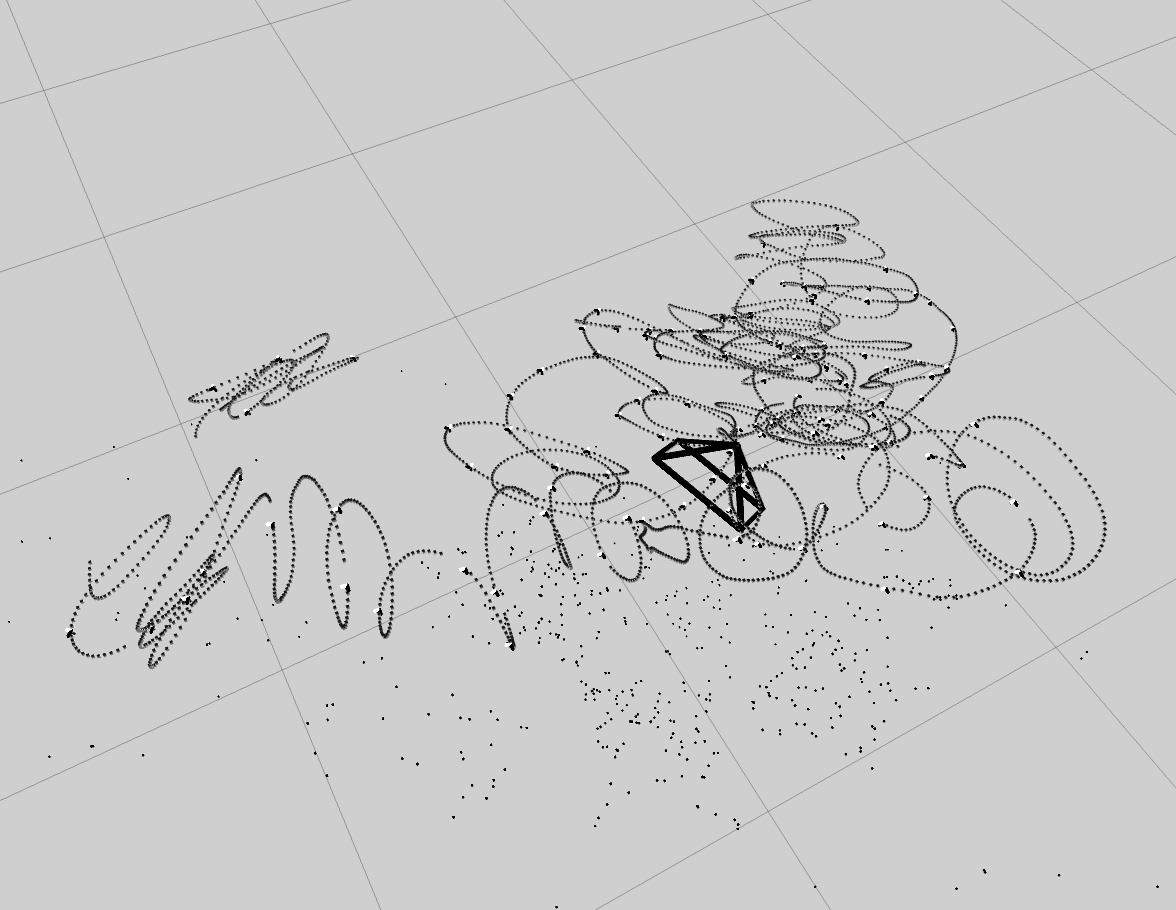
\includegraphics[scale=0.5]{img/SVO_rviz_1.png}
\caption{Vizualizace průběhu SVO v RViz.}
\end{figure}

\begin{figure}[H]
\centering
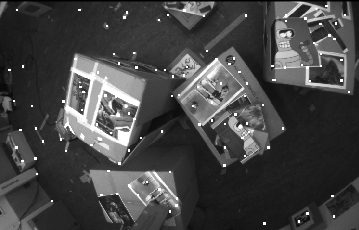
\includegraphics[scale=1]{img/SVO_rviz_2.png}
\caption{Vstupní obraz s klíčovými body SVO.}
\end{figure}

Na obrázku 11 je vykreslení ground-truth z datasetu použitého u SVO, které na první pohled moc neodpovídá trajektorii. Na obrázku 12 se nám odlišnost potvrdí, neboť i přes zarovnání trajektorie a ground-truth jsou mezi nimi velké rozdíly, avšak patrné i jistá snaha trajektorie kopírovat tvar ground-truth.

\begin{figure}[H]
\centering
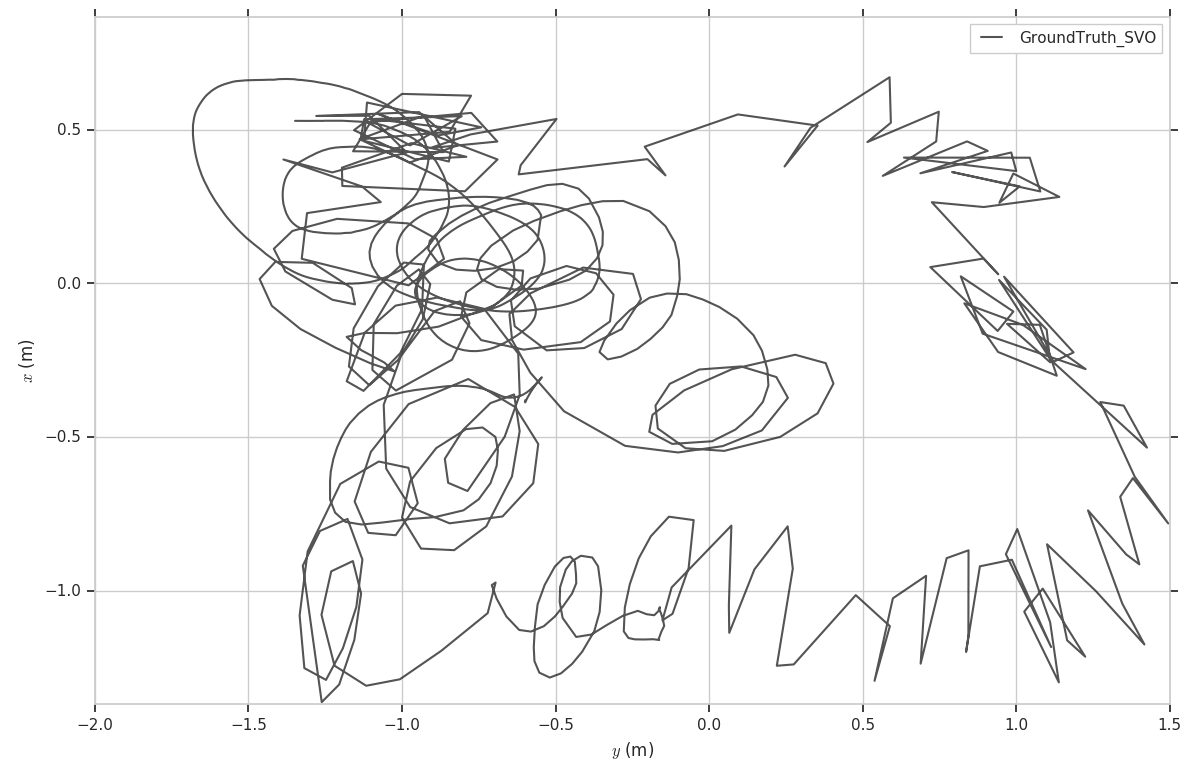
\includegraphics[scale=0.5]{img/xy_SVO_gt.png}
\caption{Vykreslení grount-truth z datasetu pro SVO.}
\end{figure}

\begin{figure}[H]
\centering
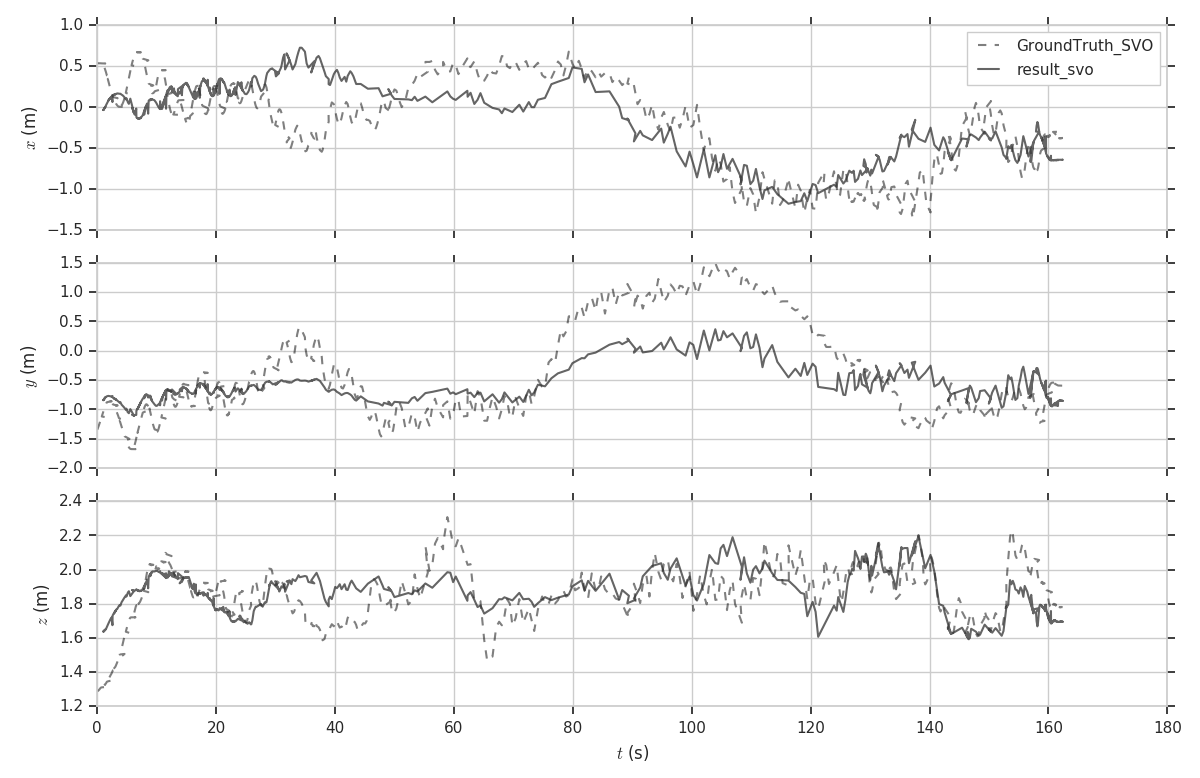
\includegraphics[scale=0.5]{img/xyz_SVO.png}
\caption{Porovnání trajektorie SVO a ground-truth}
\end{figure} 

Špatné výsledky porovnání potvrzuje i absolutní střední kvadratická odchylka, která vyšla přibližně 0,58 a relativní střední kvadratická odchylka s hodnotou 0,16m.


\subsubsection{LSD}
Large-Scale Direct Monocular SLAM ke svému běhu i instalaci vyžaduje ROS, přestože jej využívá pouze pro vstup a výstup dat. Je testován na systémech Ubuntu 12.04 s ROS Fuerte a Ubuntu 14.04 s ROS Indigo. První problémy nastaly ihned při instalaci na mnou používaný Ubuntu 16.04 s ROS Kinetic, většinou se týkaly nekompatibility verzí OpenCV, protože LSD SLAM byl vytvořen pro OpenCV verze 2, zatímco ROS Kinetic standardně používá OpenCV verze 3. K vyřešení těchto problémů, kdy LSD SLAM nemohl najít správnou cestu k OpenCV bylo zapotřebí ve složce \texttt{lsd\_slam\_core} pozměnit soubor \texttt{CMakeLists.txt} přidáním řádky
\begin{verbatim}
find_package(OpenCV REQUIRED)
\end{verbatim}
a úpravou následujících dvou příkazů
\begin{verbatim}
target_link_libraries(live_slam lsdslam 
${catkin_LIBRARIES} ${G2O_LIBRARIES})

target_link_libraries(dataset lsdslam 
${catkin_LIBRARIES} ${G2O_LIBRARIES})
\end{verbatim}
přidáním reference na knihovny OpenCV na tvar
\begin{verbatim}
target_link_libraries(live_slam lsdslam 
${catkin_LIBRARIES} ${G2O_LIBRARIES} ${OpenCV_LIBS})

target_link_libraries(dataset lsdslam 
${catkin_LIBRARIES} ${G2O_LIBRARIES} ${OpenCV_LIBS})
\end{verbatim}

Po vyřešení nekompatibility knihoven se objevila nová chyba neodpovídajících si \newline proměnných typů. Proto bylo nutné udělat změny ve zdrojovém souboru \newline \texttt{lsd\_slam\_viewer/src/PointCloudViewer.cpp} a přepsat typ proměnné na řádce 326 z \texttt{float x, y, z;} na tvar \texttt{qreal x, y, z;} a podobnou změnu udělat také v souboru \texttt{lsd\_slam\_viewer/src/PointCLoudViewer.h} a změnit řádku 135 z \texttt{float x, y, z;} na tvar \texttt{qreal x, y, z;}. Následovala již úspěšná instalace.

Spouštění LSD SLAMu se ale také neobešlo bez problémů, neboť při vizualizaci běhu algoritmu se otevře \textit{viewer} a spolu s ním \textit{DebugWindow DEPTH}, který ale ihned po otevření přestane pracovat. Algoritmus však lze do jisté míry provozovat i bez tohoto okna, které slouží pro zobrazení informací o běhu programu, vizualizaci vstupních dat s promítnutými body z LSD a spouštění některých rychlých příkazů. Jako vizualizaci tak máme k dispozici pouze husté mračno bodů tvořící 3D mapu prostředí a uraženou trajektorii.

Standardně LSD SLAM očekává vstupní data v bag souboru, obsahujícím obrazové data a kalibrační informace. Pro použití TUM datasetu je nutné algoritmu zvlášť zadat cestu k sekvenci snímků, kalibračnímu souboru a zadat informaci o frekvenci vstupního videa.

Výsledky z této metody jsem získal podobně jako u SVO, tedy s pomocí ROS topicu. Zjistil jsem, že LSD publikuje informace o poloze do \texttt{/lsd\_slam/pose} a celou trajektorii jsem zapsal do souboru spuštěním příkazu
\begin{verbatim}
rostopic echo /lsd_slam/pose > result_lsd.txt
\end{verbatim}
čímž znovu dostanu trajektorii ve formátu, který poskytuje ROS a pro potřeby dalšího vyhodnocení musím soubor převést do formátu TUM pomocí svého Python skriptu.

\subsubsection*{Výsledky}
Ukázalo se, že LSD SLAM neimplementuje žádnou možnost získání globální trajektorie a můj způsob extrakce za pomocí ROS získává pouze relativní trajektorii se špatným měřítkem, která navíc ani neprošla optimalizací. Metoda tedy podle vizualizace funguje správně, ale výslednou trajektorii jsem nedokázal extrahovat ani při úpravách zdrojových souborů.

Na obrázku 13 je porovnání trajektorií z LSD (s ručně upraveným měřítkem) a LDSO na stejném datasetu a lze pozorovat jistou podobnost i napříč relativními daty z LSD a absolutními daty z LDSO. Explicitně porovnat mezi sebou nebo oproti ground-truth je však nelze.

\begin{figure}[H]
\centering
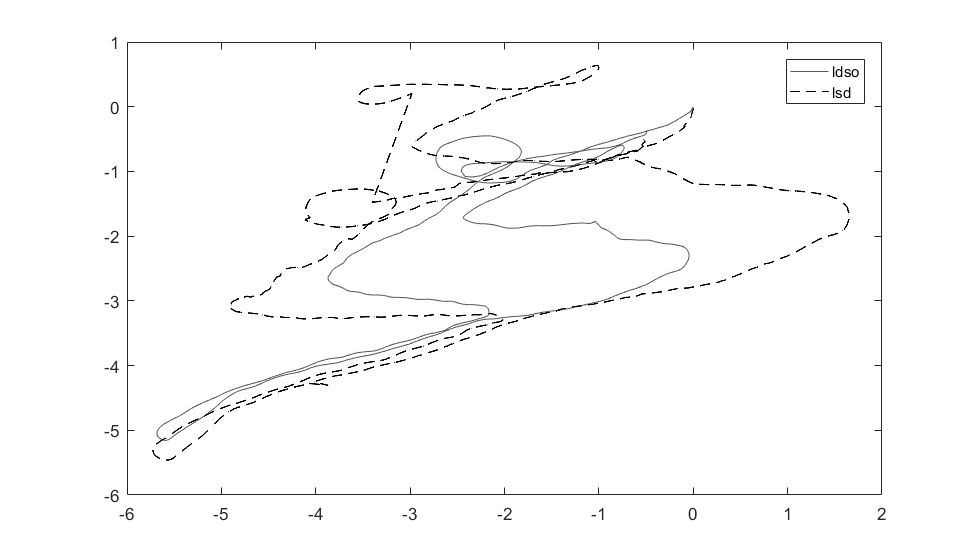
\includegraphics[scale=0.62]{img/porov_lsd_ldso.png}
\caption{Porovnání trajektorie z LDSO a upravené trajektorie z LSD.}
\end{figure} 

\begin{figure}[H]
\centering
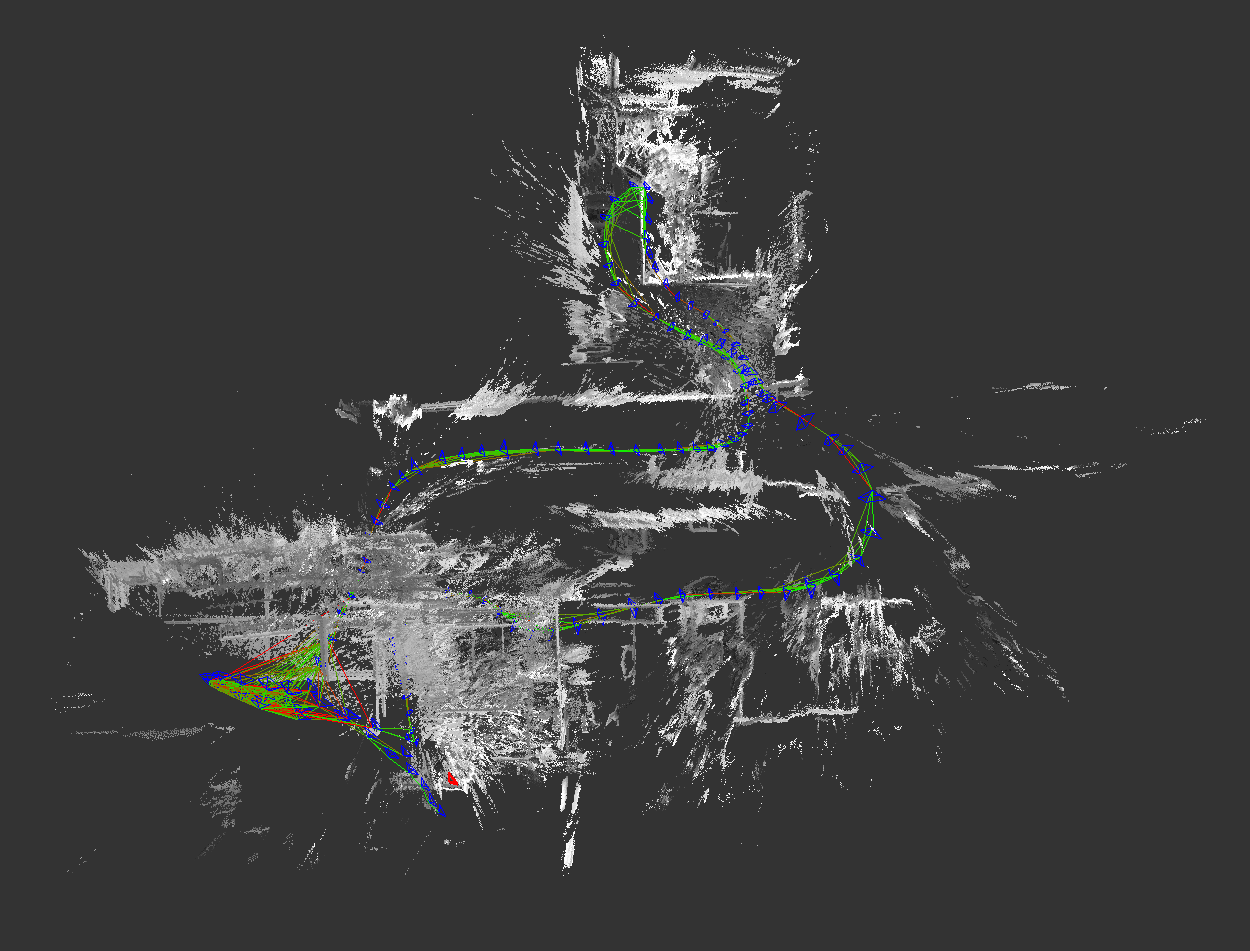
\includegraphics[scale=0.455]{img/LSD_11_top.png}
\caption{.}
\end{figure} 

\begin{figure}[H]
\centering
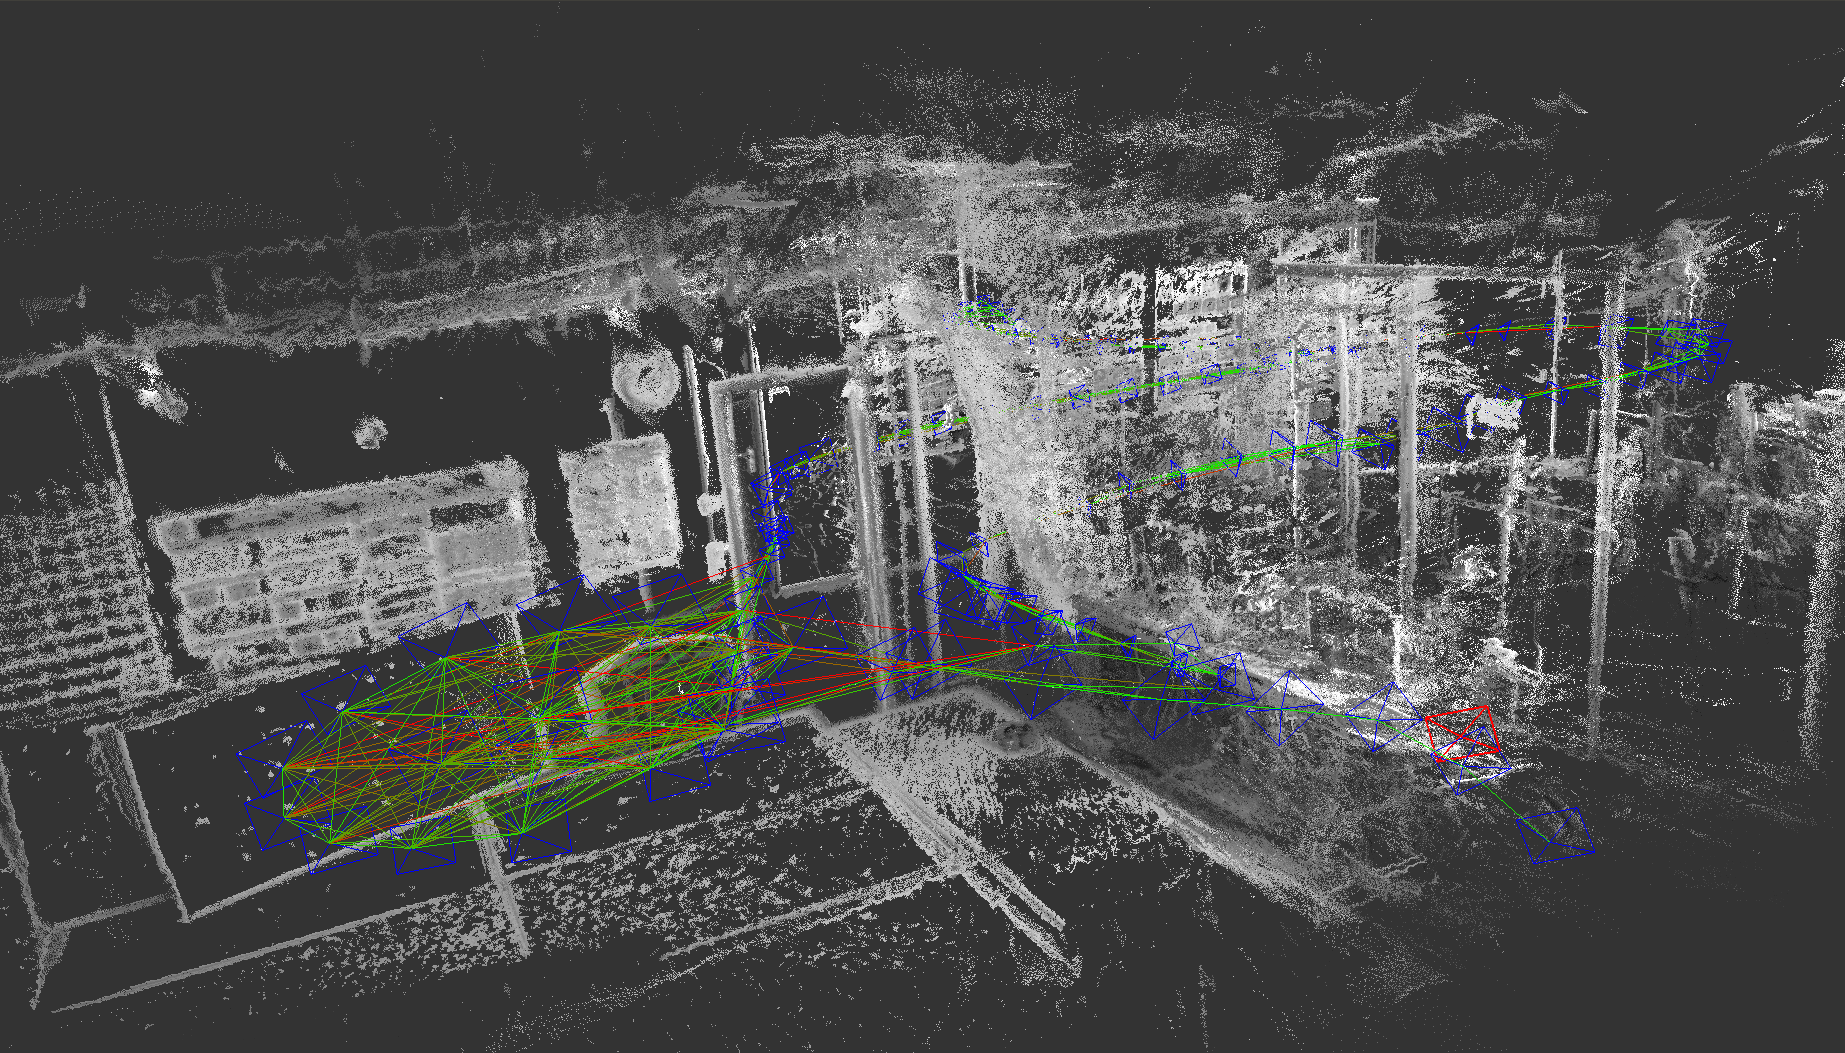
\includegraphics[scale=0.31]{img/LSD_11_kancl.png}
\caption{.}
\end{figure} 

\subsubsection{DSO}

\subsubsection{LDSO}






\textsf{\textbf{TODO-----------------------------------------------------------}}

úprava LoopClosing.cc a následná rekompilace u LDSO pro fungování OpenCV3. Zkontrolovat, jestli to doopravdy dělá loopclosing, nebo jen obchází problém.

https://github.com/tum-vision/LDSO/issues/21


\bibliography{zdroje}




\end{document}

